\section{An infrastructure for non-functional testing using docker containers
technologies}

To facilitate the testing of code generators, we need to deploy produced binaries on an elastic infrastructure that
provides preconfigured virtual server images, storage and network connectivity that may be
provisioned by testers. Monitoring information should also be provided to inform about resource utilization required/needed and to automate the resource management. For this purpose, we propose a testing infrastructure based on docker environment. 

Docker will automate the deployment of applications inside software containers. It will simplify the creation
of highly distributed systems by allowing multiple applications to run autonomously on a server
(basically a cloud server). Docker will provide a platform as a service (PaaS) style of
deployment for software programs. Consequently, we will rely on this technology and benefit from all its advantages to:
\begin{enumerate}
	\item Deploy preconfigured application to test within docker containers
	\item Automate optimization sequences generation
	\item Monitor service containers
	\item Gather performance metrics (CPU, Memory, I/O, etc.)
\end{enumerate}
As a consequence, we are going to integrate a collection of docker technologies to define the adequate infrastructure for testing and monitoring code generators. So which docker technologies must be glued together? and how can we integrate our NS optimizations generator within this architecture?

In the following,  we will describe how can we ease the deployment and configuration of generated code within docker.
\subsection{Docker as a deployment environment}
Before starting monitoring and testing applications, we have to deploy different applications on different components to ease containers provisioning and profiling.
We aim to use Docker Linux containers to monitor the execution of produced binaries by GCC compilers in term of resource usage. 
Docker is an open source engine that automates the deployment of any application as a
lightweight, portable, and self-sufficient container that will run virtually on host machine. To achieve that, Docker uses the Linux container technology. The main advantages that Docker offers compared to using a full stack virtualization solution is less performance overhead and resource isolation.

Using docker, we can define preconfigured applications and servers to host. We can also define the way the service should be deployed in the host machine. As properties, we can define the OS where the service has to run, dependencies, etc. Once docker images are defined, we can instantiate different containers.

A simple way to define docker images is to use dockerfiles. Docker can build images automatically by reading the instructions from a Dockerfile. Therefore, for our experiments we describe a dockerfile that defines the target compiler to test, as well the container OS. The same docker image will be used then to execute different instances of generated code.

Docker uses as well Linux control groups to group processes running in the container. This allows us to manage the resources of a group of processes, which is very valuable. This approach gives a lot of flexibility when we want to manage resources, since we can manage every group individually. 

Therefore to run our experiments, each optimized program is executed individually inside an isolated Linux container. By doing so, we ensure that each executed program runs in isolation without being affected by the host machine or any other processes. Moreover, since a container is cheap to create, we will be able to create too many containers as long as we have new programs to execute and the system does not suffer too much from the performance trade-off.

Since each program execution requires a new container to be created, it is crucial to remove and kill containers that have finished their job to eliminate the load on the system. In fact, containers/programs are running sequentially without defining any constraints on resource utilization for each container. So once execution is done, resources reserved for the container are automatically released to enable spawning next containers.

\subsection{Monitoring components}
Docker containers rely on control groups (cgroups) to expose a lot of metrics about accumulated CPU cycles, memory, and block I/O usage. In order to achieve docker monitoring of our running applications within docker containers, we aim to use some docker facilities to ease the extraction of performance metrics.
\subsubsection{Monitoring component: cAdvisor}
So, we use google containers called cAdvisor as Container Advisor\footnote{https://github.com/google/cadvisor}. It is a tool developed by Google to monitor their infrastructure. This container will provide us an understanding of the resource usage and performance characteristics of our running containers. In fact, it automates the extraction of performance metrics using cgroups file systems at runtime. Thus, cAdvisor collects, aggregates, processes, and exports information about running containers. We note that resource usage information is collected in raw data.

cAdvisor does not need any configuration on the host machine. We have just to run cAdvisor container on our docker host. It will then have access to the resource usage and performance characteristics of all running containers. For example, cAdivsor accesses at runtime to CPU consumption metrics available at the cgroup file system via stats found in $/sys/fs/cgroup/cpu/docker/(longid)/$ and reports all statistics via web UI ($http://localhost:8080$) to view live resource consumption for each container. Stats related to memory consumption can be found as well in $/sys/fs/cgroup/memory/docker/(longid)/$. cAdvisor will automate the process of service discovery and metrics aggregation so that, instead of gathering manually metrics located in cgroups file systems we will use it to ease this task. It has been widely in different projects namely Heapster\footnote{https://github.com/kubernetes/heapster} and Google Cloud Platform\footnote{https://cloud.google.com/}.

cAdvisor may induce a little overhead, because it does very fine-grained accounting of the memory usage on running container. This is may not affect the gathered performance values since we run only one generated program by GCC within each container.

cAdvisor monitors and aggregates data over only 60 seconds interval. It collects ephemeral data in real-time for each container. This limitation can in many cases be overseen but we would like to record all data over time. This is useful to execute queries and define metrics from historical data. Thereby, To make gathered data from cAdvisor truly valuable for monitoring resources usage, it becomes necessary to log it in a database at runtime. Fortunately, cAdvisor can easily be plugged together with a database.
\subsubsection{Back-end Database component: InfluxDB}
We use InfluxDB\footnote{https://github.com/influxdata/influxdb}, an open source distributed time series database as backend to record data. It collects docker container performance metrics through cAdvisor for long-term retention, analytics and visualization. When a new container is launched it will be automatically fetched by cAdvisor and its statistics will be continuously sent into InfluxDB while the container is running. When a container is killed, all statistics will be deleted afterward. cAdvisor must be plugged with the new created
times-series database created in influxDB to use it as a datastore back-end. Hence, we add the ip port of the database to cadvisor image. So, container statistics are sent over TCP port (e.g, 8086) exposed by influxdb.
InfluxDB allow the user to execute SQL queries on the database. For example the following query reports the average memory usage of container $"generated-code-v1"$ for each 2s since container has been started:

\begin{lstlisting}[
language=SQL,
showspaces=false,
basicstyle=\ttfamily,
numbers=left,
numberstyle=\tiny,
commentstyle=\color{gray}
]
select mean(memory_usage) from stats where 
container_name='generated-code-v1' group by 
time(2s)
\end{lstlisting}
To give an idea about data stored in InfluxDB. The following table describes the different performance metrics stored in InfluxDB:
 \begin{table}[h]
 	\begin{center}
 		\begin{tabular}{|p{1cm}|p{6.9cm}|}
 			\hline
 			 Name & Name of the container \\
 			\hline
 			 Ts & Starting time of the container in epoch time (seconds) \\
 			\hline
 			 Network &  Stats for network bytes and packets in an out of the container \\
 			\hline
 			 Disk IO &  Disk I/O stats for the container \\
 			\hline
 			 Memory &  Memory usage in KB \\
 			
 			\hline
 		   	CPU &  Cumulative CPU usage \\
 			\hline
 			
 		\end{tabular}
 		
 	\end{center}
 	\caption {Resource usage metrics recorded in InfluxDB}
 \end{table}
For the moment, we set our back-end for docker monitoring tool (cAdvisor+influxDB). It would be nice to pull all the pieces together visually to view nice charted graphs within a complete dashboard. It is relevant to show performance profiles of memory and CPU consumption of our running applications overtime. To do that, we present Grafana for performance profiling. 

\subsubsection{Front-end Visualization Component: Grafana}
Once we have gathered and stored performance data, the next step is visualizing them. That is the role of Grafana\footnote{https://github.com/grafana/grafana}. Grafana can be considered as a web application running within a container. It is one of the best time-series metric visualization tools available. It can easily work with data held in InfluxDB. It provides us a dashboard to run queries against the linked database and chart them accordingly in a very nice layout. Grafana will be the endpoint that we will use to visualize the recorded data. It is easily configurable and will let us choose what to render through Web UI. We run Grafana within a docker container and we link it to InfluxDB by setting the data port 8086 so that it can easily request data from the database.

We recall that influxDB has also an interface to query the database and show graphs. But, Grafana let us store our searches and display the results in much pretty looking graphs. That is why we used Grafana.
As well, we can set up the profile of resource consumption for different running
containers. Thereby, we can compare the profile of CPU and memory consumption among containers. The only thing we have to care about is the metric definitions (using SQL queries like in InfluxDB). Once we define which data we have to extract from the database for visualization, we can draw up whatever we want using Grafana dashboard. Finally, we can save the created dashboard as well as all its dependencies like the defined metrics, database source... We can also export the data currently being viewed within different
panels into static JSON or CSV document. Thereby, we can perform statistical analysis on this data to detect bugs or performance anomalies.

\subsection{Wrapping everything together: Architecture Overview}
To summarize, we present, as shown in Figure 1, an overall overview of the different components involved in our docker monitoring infrastructure.

Our testing infrastructure will run different jobs within docker containers. First, we generate and run different versions of code using our target compiler. To do so, we run multiple instances of our preconfigured docker image that corresponds to specific code generator (e.g, GCC compiler). Each container will execute a specific job for the input program. For our case, a job represents a program compiled with new optimization sequence generated by NS. In the meanwhile, we run our monitoring components (cAdvisor, InfluxDB and Grafana). cAdvisor collects usage statistics of all running containers and save them at runtime in the time series database InfluxDB. Grafana comes later to allow the end users to define performance metrics and draw up charts.
\begin{figure}[h]
	\centering
	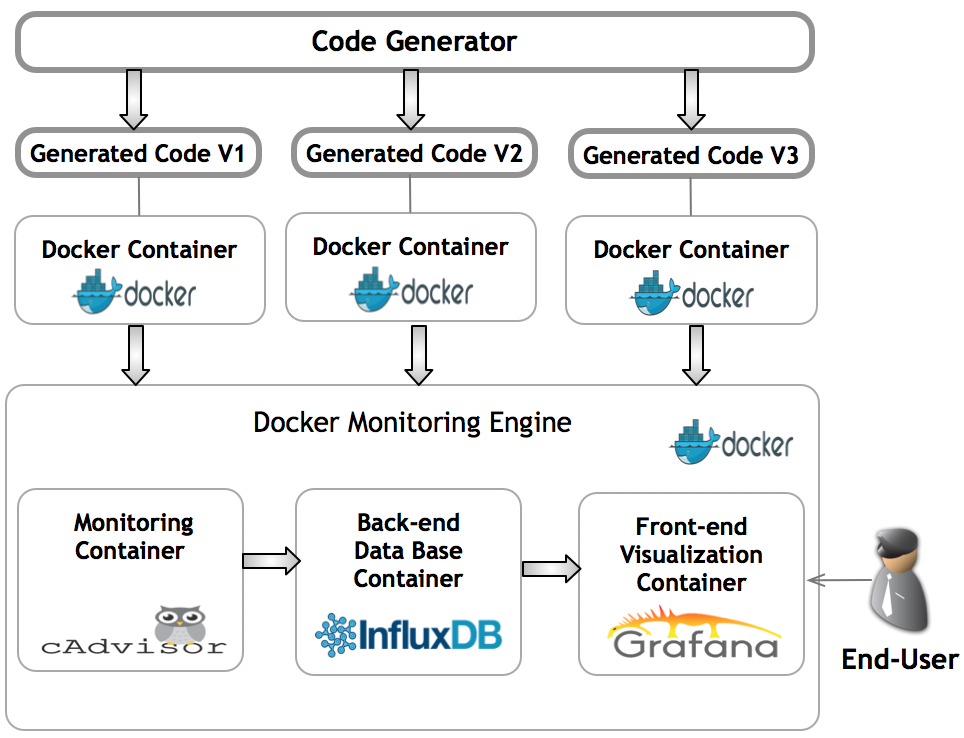
\includegraphics[scale=0.50]{Ressources/infra.png}
	\caption{Overview of the docker-based testing architecture}
\end{figure}